\documentclass{article}

\usepackage{tikz}
\usetikzlibrary{math}

\usepackage{xcolor}

\usepackage{hyperref}
\hypersetup{
    pdftitle={Easy colorblind-safe typesetting: the colorblind package},
    pdfauthor={Simon Pfahler},
}
\usepackage{cleveref}

\usepackage{csquotes}
\usepackage[backend=biber, style=numeric-comp, seconds=true, sorting=none, subentry=true, doi=false, alldates=iso]{biblatex}
\renewcommand*{\entrysetpunct}{\\[5pt]}
\addbibresource{bib.bib}

\usepackage{colorblind}

\title{Easy colorblind-safe typesetting:\\ the \textbf{colorblind} package}
\author{Simon Pfahler}
\date{\today}

\begin{document}

\maketitle

\section{Provided color schemes}

\subsection{Paul Tol's color schemes}

\begin{figure}[ht]
    \centering
    \drawScheme{T_Q_B}
    \caption{Bright qualitative color scheme by Paul Tol~\cite{Tol}.}
    \label{fig:T_Q_B}
\end{figure}






\section{Experimental and work in progress}

\let\oldcolor\color

\newcommand\normalvision{%
    \protect\renewcommand\color[1]{\oldcolor{##1}}%
}

\newcommand\protanopia{%
    \protect\renewcommand\color[1]{%
        \extractcolorspecs{##1}{\modelspec}{\colorspec}%
        \tikzmath{
            \r = array({\colorspec},0);
            \g = array({\colorspec},1);
            \b = array({\colorspec},2);
            \rp = pow(0.06425 + 0.677*pow(\g, 2.2) + 0.2802*pow(\r, 2.2), 1./2.2);
            \gp = pow(0.06425 + 0.677*pow(\g, 2.2) + 0.2802*pow(\r, 2.2), 1./2.2);
            \bp = pow(0.06425 + 0.95724*pow(\b, 2.2) + 0.02138*pow(\g, 2.2) - 0.02138*pow(\r, 2.2), 1./2.2);
        }%
        \oldcolor[rgb]{\rp,\gp,\bp}%
    }%
}

\newcommand\deuteranopia{%
    \protect\renewcommand\color[1]{%
        \extractcolorspecs{##1}{\modelspec}{\colorspec}%
        \tikzmath{
            \r = array({\colorspec},0);
            \g = array({\colorspec},1);
            \b = array({\colorspec},2);
            \rp = pow(0.01194 + 0.8806*pow(\g, 2.2) + 0.1115*pow(\r, 2.2), 1./2.2);
            \gp = pow(0.01194 + 0.8806*pow(\g, 2.2) + 0.1115*pow(\r, 2.2), 1./2.2);
            \bp = pow(0.01194 + 0.992052*pow(\b, 2.2) - 0.003974*pow(\g, 2.2) + 0.003974*pow(\r, 2.2), 1./2.2);
        }%
        \oldcolor[rgb]{\rp,\gp,\bp}%
    }%
}

\begin{figure}[ht]
    \centering
    \begin{tikzpicture}
        \newcommand{\dx}{1}
        \newcommand{\dy}{-1.5}
        \newcommand{\radius}{0.7}

        % test for non rgb color models
        \definecolor{hsbtest1}{rgb}{0.266, 0.465, 0.664}
        \definecolor{hsbtest2}{hsb}{0.266, 0.468, 0.664}
        
        % Tol's bright qualitative color scheme
        \fill[T_Q_B1] (0,0) circle (\radius);
        \fill[T_Q_B2] (\dx,0) circle (\radius);
        \fill[T_Q_B3] (2*\dx,0) circle (\radius);
        \fill[T_Q_B4] (3*\dx,0) circle (\radius);
        \fill[T_Q_B5] (4*\dx,0) circle (\radius);
        \fill[T_Q_B6] (5*\dx,0) circle (\radius);
        \fill[T_Q_Bgrey] (6*\dx,0) circle (\radius);

        \fill[hsbtest1] (8*\dx,0) circle (\radius);
        \fill[hsbtest2] (9*\dx,0) circle (\radius);
        
        {
        \protanopia
        \fill[T_Q_B1, rounded corners=0.7*\radius cm]
            (0-\radius,\dy-0.7*\radius) rectangle ++(2*\radius, 1.4*\radius);
        \fill[T_Q_B2, rounded corners=0.7*\radius cm]
            (\dx-\radius,\dy-0.7*\radius) rectangle ++(2*\radius, 1.4*\radius);
        \fill[T_Q_B3, rounded corners=0.7*\radius cm]
            (2*\dx-\radius,\dy-0.7*\radius) rectangle ++(2*\radius, 1.4*\radius);
        \fill[T_Q_B4, rounded corners=0.7*\radius cm]
            (3*\dx-\radius,\dy-0.7*\radius) rectangle ++(2*\radius, 1.4*\radius);
        \fill[T_Q_B5, rounded corners=0.7*\radius cm]
            (4*\dx-\radius,\dy-0.7*\radius) rectangle ++(2*\radius, 1.4*\radius);
        \fill[T_Q_B6, rounded corners=0.7*\radius cm]
            (5*\dx-\radius,\dy-0.7*\radius) rectangle ++(2*\radius, 1.4*\radius);
        \fill[T_Q_Bgrey, rounded corners=0.7*\radius cm]
            (6*\dx-\radius,\dy-0.7*\radius) rectangle ++(2*\radius, 1.4*\radius);

        \fill[hsbtest1, rounded corners=0.7*\radius cm]
            (8*\dx-\radius,\dy-0.7*\radius) rectangle ++(2*\radius, 1.4*\radius);
        \fill[hsbtest2, rounded corners=0.7*\radius cm]
            (9*\dx-\radius,\dy-0.7*\radius) rectangle ++(2*\radius, 1.4*\radius);

        }
        
        {
        \deuteranopia
        \fill[T_Q_B1, rounded corners=0.7*\radius cm]
            (0-\radius,1.8*\dy-0.7*\radius) rectangle ++(2*\radius, 1.4*\radius);
        \fill[T_Q_B2, rounded corners=0.7*\radius cm]
            (\dx-\radius,1.8*\dy-0.7*\radius) rectangle ++(2*\radius, 1.4*\radius);
        \fill[T_Q_B3, rounded corners=0.7*\radius cm]
            (2*\dx-\radius,1.8*\dy-0.7*\radius) rectangle ++(2*\radius, 1.4*\radius);
        \fill[T_Q_B4, rounded corners=0.7*\radius cm]
            (3*\dx-\radius,1.8*\dy-0.7*\radius) rectangle ++(2*\radius, 1.4*\radius);
        \fill[T_Q_B5, rounded corners=0.7*\radius cm]
            (4*\dx-\radius,1.8*\dy-0.7*\radius) rectangle ++(2*\radius, 1.4*\radius);
        \fill[T_Q_B6, rounded corners=0.7*\radius cm]
            (5*\dx-\radius,1.8*\dy-0.7*\radius) rectangle ++(2*\radius, 1.4*\radius);
        \fill[T_Q_Bgrey, rounded corners=0.7*\radius cm]
            (6*\dx-\radius,1.8*\dy-0.7*\radius) rectangle ++(2*\radius, 1.4*\radius);
        
        \fill[hsbtest1, rounded corners=0.7*\radius cm]
            (8*\dx-\radius,1.8*\dy-0.7*\radius) rectangle ++(2*\radius, 1.4*\radius);
        \fill[hsbtest2, rounded corners=0.7*\radius cm]
            (9*\dx-\radius,1.8*\dy-0.7*\radius) rectangle ++(2*\radius, 1.4*\radius);
        }
    \end{tikzpicture}
    \caption{Test for deuteranopia and tritanopia commands: Left shows Tol's bright qualitative scheme, with deuteranopia and tritanopia vision in the second and third row. Right shows two colors with the same numbers in rgb and hsb, where the hsb variant gets translated incorrectly to color-deficient visions.}
\end{figure}

\begin{figure}[ht]
    \centering
    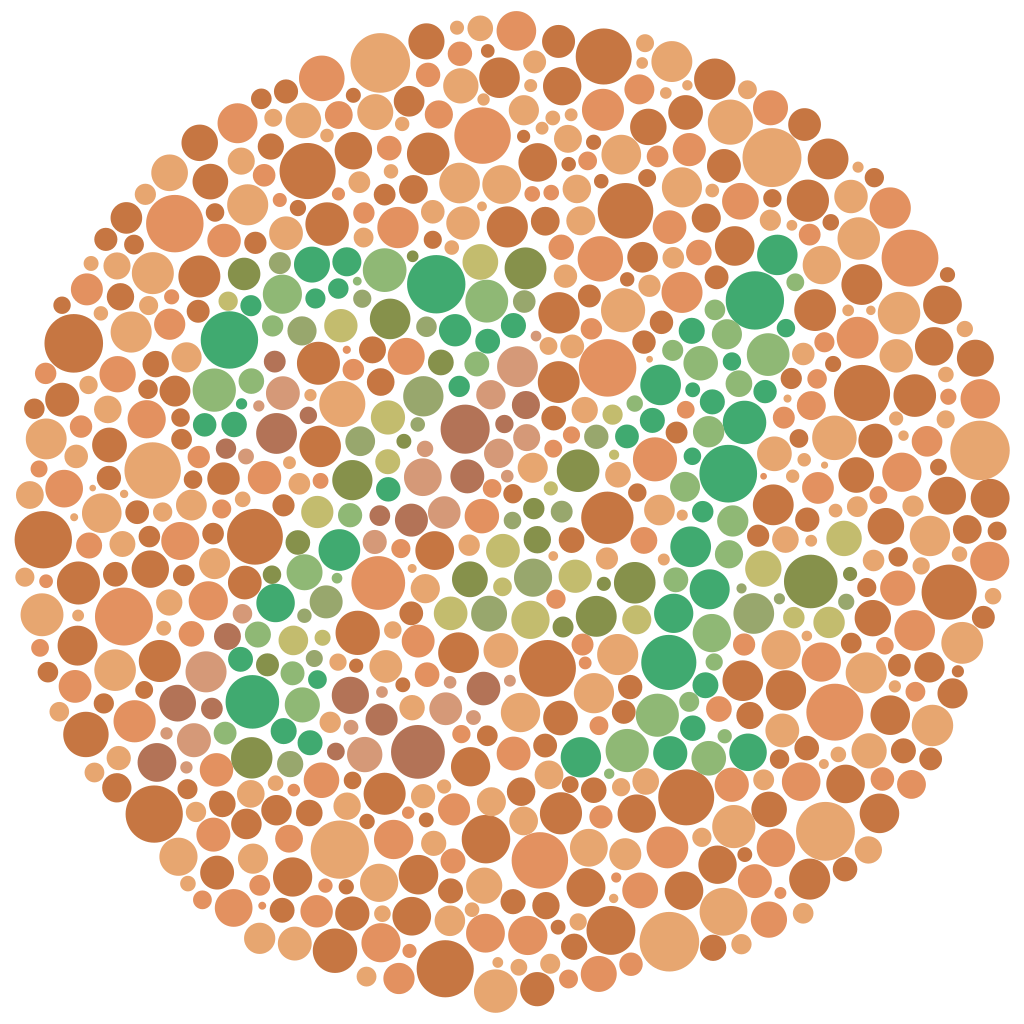
\includegraphics[width=0.3\textwidth]{Ishihara_9.png}
    \hspace{1cm}
    {\selectcolormodel{gray}
        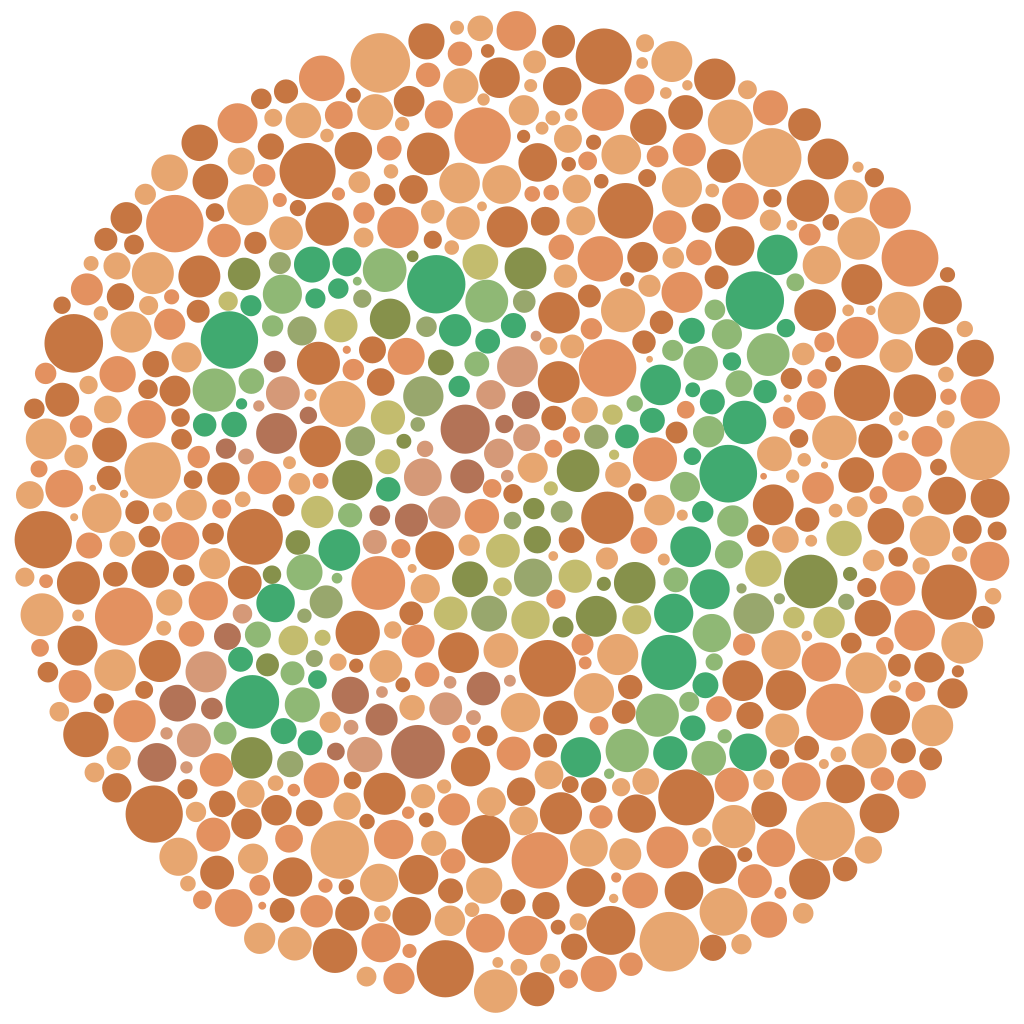
\includegraphics[decodearray={0 0 0 1 0 1}, width=0.3\textwidth]{Ishihara_9.png}
    }
    \caption{Ishihara colorblindness test, normal vision and without the {\color{red}red} channel.}
\end{figure}

\printbibliography

\end{document}
